\section{The Order Is in the Program}
\label{sec:order}

% VALUE: on XDNA 2 each engine runs its program in order and nothing schedules across engines, so the order of the work and the waits between engines are in the compiled program; the section shows this from measured command semantics, states the execution model, reads a stream into a happens-before graph with a cause per wait, and extends the reading to closed binaries
On XDNA~2, each engine runs its own program in order, and no hardware or runtime scheduler reorders work across engines, while arbitration on shared ports and locks serializes work at run time and enters the analysis as a resource.
The order of the work and the waits between engines are therefore fixed by the compiled program and the host's dispatch sequence, whereas their durations are not.
We first establish how the CP turns instruction streams into concurrency (Section~\ref{subsec:semantics}), then state the execution model the analysis assumes (Section~\ref{subsec:model}), read a stream into a graph of what must finish before what starts, with a cause for each wait (Section~\ref{subsec:reading}), and extend the reading to binaries shipped without source (Section~\ref{subsec:closed}).

\subsection{Command Semantics}
\label{subsec:semantics}

% VALUE: the CP semantics, measured on the existing prefill's own operators, say where concurrency can come from: not from queued commands, but from one command that issues both groups' work before it waits on either
To find where concurrency can come from, we measure how the CP turns instruction streams into overlap on the existing prefill's own operators, pairing one attention operator on columns 0 and 7 with one GEMM operator on columns 1--6.
Every composed command here produces outputs bit-identical to those of the operators run alone.

\begin{figure}[t]
    \centering
    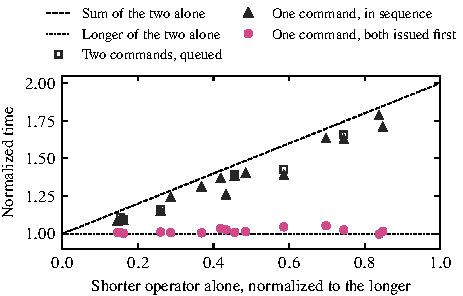
\includegraphics[width=\linewidth]{fig/pairs.pdf}
    % VALUE: queued commands take the sum of the two operators, one command that issues both before waiting takes the longer one
    \caption{Median time of one attention and one GEMM operator on disjoint column groups, normalized to the longer operator alone, over 20 runs per pair. Holding both streams in one command saves one dispatch floor against the sum.}
    \label{fig:pairs}
\end{figure}

\textbf{Queued Commands.}
% VALUE: the runtime gives no overlap across commands, and placing two operators in one command is itself neutral, so overlap must come from within a command
Two commands queued on one hardware context, with no wait between them, take as long as one command that holds both streams in sequence, within 3\% on every pair (Figure~\ref{fig:pairs}).
Holding both streams in sequence in one command takes the sum of the two operators' times minus one dispatch floor, within 2\%, so placing two operators in one command is itself neutral.
This is why packing several operators into one dispatch, which is standard practice for amortizing launch cost, as in CUDA Graphs~\citep{nvidia-cudagraphs}, XRT's run lists~\citep{xrt-repo}, and MLIR-AIR's multi-launch programs~\citep{wang2026mlirair}, removes dispatch cost on the NPU but creates no overlap.
% SOURCE: queued / in-sequence = 1.007-1.029 on 7 pairs (amd-npu 17f7ec3 prefill-overlap/ovl4/, lab-prefill-overlap (5)b); in-sequence / (A + G - F) = 0.996-1.021 over 17 pair runs (ovl/, ovl2/ at 8f13e05 and ovl4/; report.txt H1 column).
% SOURCE: XRT run list, /opt/xilinx/xrt/include/xrt/experimental/xrt_kernel.h:21 (XRT 2.25.0); MLIR-AIR stitch_elf (vault src-mlir-air-llms).

\textbf{Concurrent Issue.}
% VALUE: one command that issues both groups' work before it waits on either runs them concurrently at nearly the longer one's time; the small cost appears when both read DRAM near the cap
When one command issues all of the GEMM's work, then the attention operator's stream, and only then the GEMM's synchronizations, the two operators run concurrently.
Such a command takes 1.00--1.06 times the longer operator's time on 9 pairs that cover three GEMM shapes and attention over chunks 0 to 15 (Figure~\ref{fig:pairs}).
On six further pairs with other shapes and chunks, the overlap hides 90--96\% of the shorter operator's work, after excluding the dispatch floor that the merge already saves.
The overlap costs most when the pair's combined DRAM read rate approaches the read cap, at about 95\% of the cap measured in the same batch.
The serial execution of the existing prefill is therefore a property of how its commands are composed, not of the array or its configuration.
% SOURCE: interleaved / max(A, G) = 0.998-1.058 over 10 pair runs = 9 pairs (c8 + lm measured twice, 1.054 and 1.058; the figure keeps each pair's first measurement); GEMM shapes up, LM head chunk, down; attention chunks 0, 4, 8, 12, 15 (lab-prefill-overlap (3)).
% SOURCE: hidden fraction of the shorter operator's work, (in-sequence - interleaved) / (min(A, G) - F) = 0.90-0.96 on 2+qkv, 6+o, 11+gate, 14+qkv, 6+gate, 11+o (lab-prefill-overlap (5)a).
% SOURCE: DRAM rate during the interleaved command 52.2 GB/s against a same-batch 8x2 cap of 53.9-55.3 GB/s for c8 + lm, the costliest overlap (1.054-1.058) (lab-prefill-overlap (3)).

\textbf{Synchronization Order.}
% VALUE: because the CP is in order, a wait on one group delays the issue of every other group's work; the attention measurement of Section 4.1 isolates this effect, so the instruction order is a scheduling decision of its own
Since the CP executes in order, a synchronization on one group delays every later issue, including the issue of another group's work.
The existing attention operator isolates this effect (Section~\ref{subsec:losses}): its two columns carry equal work, yet alternating their segments lowers its device time to $0.67\times$ at 2{,}048 tokens with the same instructions.
The CP's instruction order, and not only the assignment of operators to commands, is therefore a scheduling decision.
% SOURCE: vault lab-prefill-overlap (4)-(5)c; Section 4.1 carries the numbers.

\textbf{Hardware Contexts.}
% VALUE: a second hardware context gives no concurrency here: the driver's source allocates every context the whole array and shares it in time, and narrower partitions would need contiguous columns, rebuilt designs, and a host round trip at every dependence, so concurrency comes from within one command
Two hardware contexts on disjoint partitions are the obvious alternative, but the driver's source shows that every hardware context on our platform is allocated all eight columns, so co-resident contexts share one partition in time.
Even where narrower partitions are allowed, a partition spans contiguous columns, whereas the existing attention sits on columns 0 and 7, so each group would need its own rebuilt design.
Every dependence between attention and a GEMM would then cross the host, which waits on one context before it submits to the other.
Concurrency on the array therefore comes from within one command, which needs no rebuild and no change to the driver or firmware.
% SOURCE: amdxdna 2.25.0 (loaded module 2.25.0_20260922, NPU Strix Halo 1022:17f0 rev 11, firmware 1.1.2.65): every firmware protocol the driver accepts on this device enables AIE2_TEMPORAL_ONLY (npu4_regs.c:94-106, the table npu5 shares), and aie2_alloc_resource (aie2_ctx.c:604-608) then requests start column 0 and all columns for every context, which the solver shares as one partition (vault lab-prefill-overlap (31)).
% SOURCE: contiguous partitions, separate 6- and 2-column builds with attention moved onto adjacent columns, and the host round trip (vault lab-prefill-overlap (1)).
% DECISION: the temporal sharing is stated from the driver's source with the driver named; a two-context behavioural check is registered and not run, so it is never worded as a measurement.

\subsection{Execution Model}
\label{subsec:model}

% VALUE: the analysis models a dispatch as operations on engines (CP instructions, BD executions, core loop iterations), each with read and write sets over locations that include every exclusively held resource; under static control one dispatch at given runtime parameters has one static set of operations, a loop with data-dependent control is reported and left out, and durations stay measured inputs
The analysis models a dispatch as operations on engines, each with a set of locations that it reads and a set that it writes.
A command contributes one operation per instruction of its stream on the CP, a DMA engine one per execution of a BD on one channel, and a core one per iteration of each counted loop.
Locations cover every resource that one operation holds exclusively, namely bytes of DRAM, memory tiles, and local memory, as well as BD slots, locks, DMA channels, task-queue slots, stream-switch ports, and configuration registers, so a structural hazard is also a conflict on a location.
For example, a lock acquire reads and writes its lock, a queue push writes a queue slot and reads its BDs, and a BD execution reads its BD slot and its source bytes and writes its destination bytes.
We assume static control: the CP's stream is straight-line, since a synchronization waits but does not branch, and every core loop is counted, with a trip count that depends on the dispatch's runtime parameters rather than on computed data.
A dispatch at given runtime parameters then has one static set of operations, and a loop with data-dependent control is reported as such and left out of the analysis.
A loop whose body holds nested control, or an access the analysis cannot classify, is likewise reported as unsupported and not analysed, which in the decode design applies to every loop outside attention.
We also assume that the host follows static control, issuing commands in an order that depends on the LLM and the lengths of the context and the prompt rather than on data, and its own work enters as a measured cost.
Durations remain measured inputs, because the program fixes the order of each engine's work but not how long the work takes \E{the per-operation costs from the microbenchmarks}.
% SOURCE: operations, locations, and static control (vault lab-cosched-passes (30), item 1); unsupported loops: 22 in the decode census build, all outside the attention herd (lab-cosched-passes (33), Limits); the host's static control (outline v9 section 1); the decode kernels' early return on the pad block branches on a runtime parameter, so it stays static per context length (lab-decode-long-context (10)).

\subsection{Reading a Stream}
\label{subsec:reading}

\begin{table}[t]
    \centering
    \caption{Ordering Mechanisms}
    \label{tab:mech}
    % VALUE: the 11 mechanisms that create a direct happens-before edge, in attribution order, with the granularity of each
    \begin{tabular*}{\linewidth}{@{\extracolsep{\fill}}rlr}
        \toprule
        \# & Mechanism & Granularity \\
        \midrule
        1 & CP synchronization and mask-poll & stream \\
        2 & CP in-order issue (completes at issue) & stream \\
        3 & Channel task queue (FIFO, depth 4) & stream \\
        4 & Dispatch order on one context & stream \\
        5 & Configuration and control-packet writes & stream \\
        6 & BD chaining and repeat & data movement \\
        7 & Locks on DMA BDs & data movement \\
        8 & Stream-switch back-pressure & data movement \\
        9 & Cascade and neighbor memory & data movement \\
        10 & Core locks & core loop \\
        11 & Core program order & core loop \\
        \bottomrule
    \end{tabular*}
\end{table}

% VALUE: happens-before is completion before start, not issue order; each direct edge comes from one of 11 mechanisms at the stream, data-movement, or loop granularity and is attributed to exactly one, and edges no mechanism explains are counted, so the count measures the model's coverage
From these operations, the analysis builds a \emph{happens-before} graph, in which an edge from $a$ to $b$ means that $b$ cannot start until $a$ has completed.
Issue order alone does not create such an edge, because a queue push is issued in order but its transfer completes later.
Each direct edge comes from one of the 11 ordering mechanisms of Table~\ref{tab:mech}, at the granularity of the CP's stream, of data movement, or of a core loop, and an edge that two mechanisms imply is attributed to the first in the table.
An operation whose ordering effect no mechanism describes, such as an unknown opcode or a write outside the known register map, takes edges to its neighbors on the CP, and counting these per stream is how the model's coverage is to be measured.
Edges of mechanism 2 never stall, because their instructions complete at issue, so they are attributed but reported apart from the blocking edges.
% SOURCE: the mechanism table, attribution order, granularities, UNATTRIBUTED, and issue edges (vault lab-cosched-passes (30), item 2); the library AIECoschedDeps (mlir-aie f1725dae1f1, pinned).

% VALUE: each direct edge is classed by the pairs of operations it alone orders: a true dependence if one is read after write, a name dependence if one is write after read or write, an order dependence otherwise; classes say whether renaming or reordering can remove the wait; a wait gating several operations is classed per gated operation, pairs ordered by two disjoint paths are counted as redundant, and data-dependent loops as control
For each direct edge, the analysis computes the pairs of operations that the edge alone orders, namely those ordered with it and not without it.
The edge is a true dependence if one of these pairs reads a location after the other writes it, a name dependence if none does but one writes after the other reads or writes, and an order dependence otherwise.
The first two follow the conflicts that Bernstein's conditions exclude between pieces of work that run in parallel~\citep{bernstein1966analysis}, and the name class covers the anti and output dependences of compilers~\citep{kuck1981dependence}.
Renaming the conflicting locations can therefore remove a name dependence, reordering can remove an order dependence, and a true dependence stays.
A synchronization that gates several operations contributes one edge per gated operation, so each operation's conflicts are classed on their own.
A pair that two disjoint paths order is lost by no single edge, so each edge on those paths may be classed as an order dependence alone, and such pairs are counted as redundant instead of being attributed to either path.
A loop with data-dependent control is counted as control.
% DECISION: this subsection states the classification the passes assume and the counts it defines, not what the committed library computes. Verified against mlir-aie f1725dae1f1 on 2026-10-21: AIECoschedDeps classifies each core loop's buffers and reports its lock edges and loop-carried distances, so the class of a wait at loop granularity is computed; the edge-level attribution, the unattributed and redundant counters, and the order class itself are not implemented there, and the order class is unreachable in that library. The stream-granularity instances this paper removes were identified by reading the designs and confirmed by measurement, and the graph of a compiled stream is built by the prefill reader rather than by the library. Every sentence here is written in that register until the attribution pass exists. The registered census of Section~\ref{subsec:census} is a DIFFERENT quantity and does not depend on this: it counts instances that the frozen scheduling pass proposes, removes and confirms, and it never classifies edges. The coverage counters owed with the attribution pass are the unattributed and redundant counts, which were never part of that census (pass-0, 2026-10-22).
Loop-carried edges are classed in the same way on the loop's iterations, with their distance recorded.
% SOURCE: classification by Lost(e), REDUNDANT, CONTROL, loop-carried distance (vault lab-cosched-passes (30), item 3).

% VALUE: the recovered order is the method and is checked through its consequences, not against a trace: removed false waits leave outputs bit-identical, measured gains stay within their bounds, and what the analysis leaves out is counted; the CP's own timer records show the issue and wait order inside each command without changing the array's configuration, and they cannot see core loops or the gaps between commands
We check the recovered order through its consequences rather than against a hardware trace.
Every wait that the analysis classes as false and that our passes remove leaves the outputs bit-identical (Section~\ref{sec:method}), each measured gain is compared with its bound (Section~\ref{subsec:tests}), and the operations that the analysis leaves out are counted per stream.
To show how the CP executes the order, we insert the runtime's record-timer instruction after each synchronization and after each run of issue instructions, so that the firmware writes an identifier and a 1.8~GHz device timer into a buffer that the host reads after the run.
The array's configuration is left unchanged.
On one 128-token prefill chunk of Llama-3.2-1B, 1{,}468 records per run leave the logits bit-identical and add no measurable device time.
For each command, they show when each column group's work was issued and how long each synchronization blocked the CP (Figure~\E{timeline}).
Between commands the timer advances at less than a tenth of its rate, so the records time intervals within a command, whereas the host's clock times the gaps between commands.
Order inside a core's loop is invisible to the CP, so the decode loop's order rests on its removal (Section~\ref{subsec:rings}).
% SOURCE: record-timer instruction TXN opcode 0x83 (12 bytes: header, size, 32-bit id; aiebu 48b69735 xaie_txn.h), XRT 2.25.0 ML Timeline (XDP 67165d6 clientDev/ml_timeline.cpp; Strix Halo listed as a client device with a debug buffer); feasibility check: split-1b-S4-L20480, 108 commands, 1,468 records per run, 5 runs with and 5 without, logits sha equal in all 10, summed start-to-wait with / without records 0.93-0.95, per-command fit of the timer 1,752-1,767 MHz against the 1,800 MHz H clock at the top DPM level (xdna-driver bc5dd96 npu4_dpm_clk_table), 110-125 M timer cycles per host second between commands (amd-npu b98e3044; vault lab-flm-streams (39), decisions log D13).
% DECISION: T-rec was withdrawn by the author (outline v9 revision 31, D13); recovery is the method in every verb row, and the timer records are a figure that governs no verb.

\subsection{Closed Binaries}
\label{subsec:closed}

% VALUE: a closed stack ships binaries only, so its streams are recorded at the runtime's boundary without the device and lifted with a byte-identical round trip; each issue is attributed to the column group its data reaches through the configuration's decoded routes; FastFlowLM's prefill then issues one group per command, and serial issue predicts its time where overlap does not
FastFlowLM ships its engines as binaries, so we record their instruction streams at the runtime's boundary, either with a recording library that never opens the device or with an interposer during a device run, and lift each stream into MLIR-AIE's runtime-sequence form.
Every stream recorded offline round-trips through the lifter byte for byte, so the analysis reads exactly what the engine dispatches.
Because FastFlowLM's attention reads through shim tiles of the GEMM columns, attributing an issue to its column would mix the groups, so the analysis decodes the configuration's stream routes and attributes each issue to the group whose compute tiles its data reaches.
Under this attribution, the one capture we analyse, a 1{,}009-token prefill of Gemma-4-E2B, changes column group only at the boundary between two commands, once into attention and once out of it in every layer, so it issues serially, one group per command.
The sum of its commands' times measured alone, each less the dispatch floor and plus the boundary cost between commands, matches its measured time within 10.0\%, inside the check's tolerance of 20.8\%, whereas full overlap would place it 36.5\% lower.
A census of which columns carry any instruction, over all 218 recorded streams and over the capture itself, agrees with this attribution without establishing it, since it counts addressed columns rather than the programs they serve; Appendix~A gives the counts.
Since FastFlowLM's closed libraries build these streams and their buffers, we measure removals on MLIR-AIR's fused prefill, which reimplements FastFlowLM's designs~\citep{wang2026mlirair}.
Its decoded configuration places the GEMMs on columns 1--6 and attention on columns 0 and 7, as FastFlowLM's fused prefill does, so the two share the column groups whose turns our passes remove.
Appendix~A states how the attribution was chosen, and what the rule registered before it labels the same capture.
% SOURCE: recording libhrx (FastFlowLM 44d01787, gemma4e-flash), every prompt length 1-1,024 recorded with 0 /dev/accel opens; 8 buckets, 218 distinct streams, round trip and identity 218 / 218 (vault lab-cosched-passes (14)); lifter fix mlir-aie 91f64387ffb, 375 / 375 MLIR-AIR streams byte-identical (lab-cosched-passes (3)).
% SOURCE: device capture through an XRT interposer, gemma4e-flash:e2b, 1,009 tokens; route maps from the frozen cdo_routes decoder: shim 3 and shim 6 MM2S0 reach only columns 0 and 7; 70 group transitions, all between commands (35 GEMM -> attention, 35 attention -> GEMM) (vault lab-flm-streams (11), (13)).
% SOURCE: ops-per-column census over the 218 FLM streams, recomputed here from the committed artifact (aie-cosched 0400fc9 passes/results/bprime/column_ops.json, from bprime_column_ops.py 879bf80; parsed by aie-cosched-pass-0, counts re-derived independently in this workspace): column sets {1,2,3,4,5,6} 200, {0,3} 8, {6,7} 8, {} 1, all eight 1. Every {0,3} stream carries the bulk of its ops on column 0 (e.g. 1,420 against 384) and every {6,7} on column 7, which matches the frozen route map above (shim 3 and shim 6 MM2S0 reach only columns 0 and 7), so the 16 are attention commands plus their feeding shim. The peer's first message said 192 of 218 and corrected it to 200; 192 is the count among proposal streams only. The one empty stream (186fd90831c87d8c) was earlier reported as "not analysed: one column" and in fact has no ops.
% SOURCE: closed-stack check: T = 1.444 s, serial prediction 1.300 s (error 0.100), overlap prediction 0.917 s (error 0.365), tolerance 0.2075, of which 0.102 is one slow floor repetition; without it the tolerance is 0.106 and the serial prediction still passes (vault lab-flm-streams (12) RESULT, amd-npu 52c8401d, 3d0d1036).
% SOURCE: MLIR-AIR's llms README: "reimplement AMD NPU LLM designs originally developed by the FastFlowLM team" (mlir-air 740cae0f, a3e26261); fused_prefill/device.py "laid out like FastFlowLM's fused_prefill"; FastFlowLM's Gemma4-E2B fused_prefill.xclbin decoded with tools/xclbin_layout.py: attention programs on columns 0 and 7, a GEMM program on the 24 cores of columns 1-6 (vault lab-flm-streams (5)); coverage ruling D13(b).
% DECISION: the serial label is scoped to this one capture (Gemma-4-E2B, 1,009 tokens, the engine's cap); the attribution by routes was ruled after the capture, and the label under the first attribution by tile column was MIXED-majority; both disclosures go to the appendix (outline v9 section 2, C2).
